\section{Multistep Method}

\subsection{Observations}
\begin{frame}
	\frametitle{FW-BW Algorithm}
	\begin{itemize}
		\setlength\itemsep{1em}
		\item[Pros] It be efficient if a graph has relatively small number 
			of large and equall-sized SCCs.
		\item[Cons] Work imbalance after the large SCC is found.
	\end{itemize}
\end{frame}

\begin{frame}
	\frametitle{Coloring Algorithm}
	\begin{itemize}
		\setlength\itemsep{1em}
		\item[Pros] It be efficient if a graph has a large number of samll
			and disconnected SCCs.
		\item[Cons] Poor initial performance on real-world graphs.
	\end{itemize}
\end{frame}

\subsection{Multistep Method}
\begin{frame}
	\frametitle{Multistep Method}
	\begin{figure}
		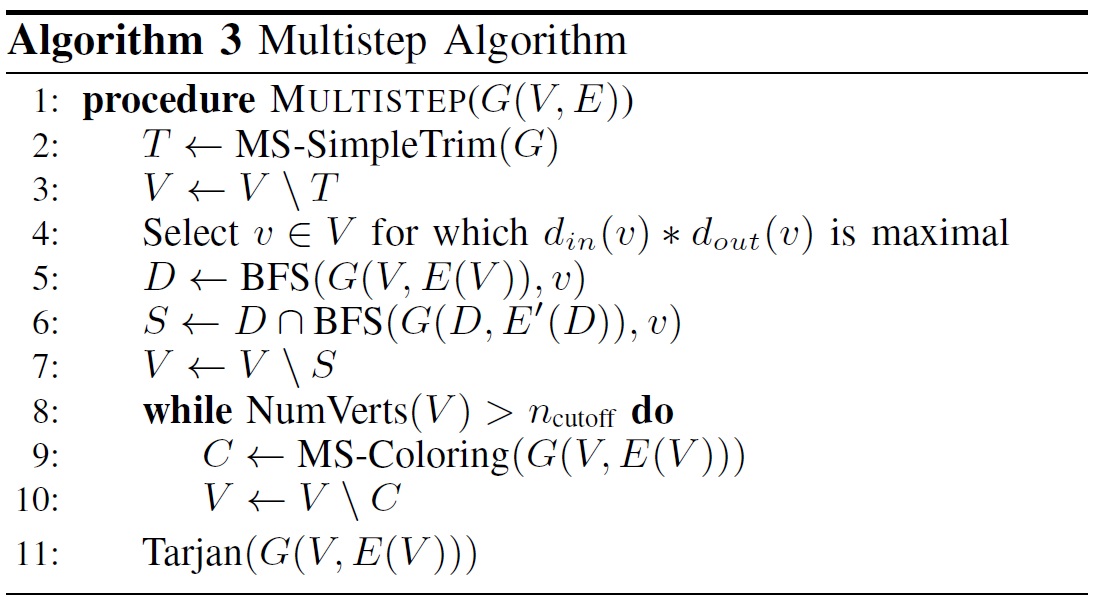
\includegraphics[scale=0.30]{figure/fig-Multistep.png}
	\end{figure}
\end{frame}

\subsection{Serial Complexity}
\begin{frame}
	\frametitle{Serial Complexity}
	\begin{itemize}
		\setlength\itemsep{0.5em}
		\item \texttt{MS-SimpleTrim(G)}
			\begin{itemize}
				\item Naive complete trimming will trim one vertex over each 
					of $n$ iterations, resulting in an upper bound of 
					$O(n^2)$ work.
				\item It uses simple trimming, or performing only a single pass
					resulting in $O(n)$ work.
			\end{itemize}
		\item \texttt{MS-Coloring(G(V,E(V)))}
			\begin{itemize}
				\item The Upper bound of naive coloring is $O(n^2)$.
				\item It uses a predefined cutoff to switch to the 
					serial algorithm.
			\end{itemize}
	\end{itemize}
	The worst case instance for Multistep will be a mostly acycle graph,
	and this would require $O(n^2)$ work.
\end{frame}
